\subsubsection{UC - Creazione di una prenotazione}

\begin{figure}[h]
  \centering
    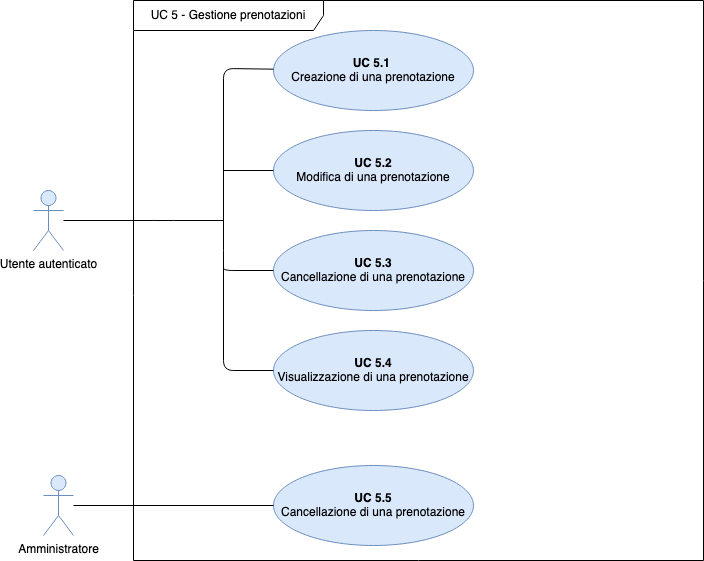
\includegraphics[scale=0.5]{src/CasiDUso/Immagini/UC5.png}
  \caption{UC  - Creazione di una prenotazione}
\end{figure}

Il presente diagramma vuole riassumere la possibilità di gestione delle prenotazioni da parte di un utente autenticato nell’applicazione.

\begin{itemize}
\item \textbf{Attori primari:} personale interno autenticato;
\item \textbf{Descrizione:} il personale interno autenticato vuole gestire una prenotazione a cui ha accesso a livello di permessi, con possibilità di creazione, modifica, eliminazione e visualizzazione;
\item \textbf{Precondizione:} il personale interno è autenticato nell’applicazione e ha i permessi per eseguire le azioni di cui sopra;
\item \textbf{Postcondizione:} il personale interno autenticato ha creato, modificato, eliminato o visualizzato una prenotazione;
\item \textbf{Scenario principale:} 
	\begin{itemize}
		\item il personale interno naviga nell’apposita sezione di modifica della prenotazione;
		\item il personale interno crea, visualizza, modifica o rimuove una sua prenotazione;
		\item la prenotazione passa in stato di “pending” e, dopo una serie di controlli, viene confermata o eliminata.
	\end{itemize}
\end{itemize}

\subsubsection{UC 1 - Creazione di una prenotazione}

\begin{itemize}
\item \textbf{Attori primari:} personale interno autenticato;
\item \textbf{Descrizione:} il personale interno autenticato vuole prenotare una postazione per una certa data od orario;
\item \textbf{Precondizione:} il personale interno è autenticato e naviga nell’apposita sezione di creazione di una prenotazione;
\item \textbf{Postcondizione:} il personale interno autenticato crea correttamente una prenotazione per la data ed ora scelta;
\item \textbf{Scenario principale:} 
	\begin{itemize}
		\item il sistema elabora correttamente la richiesta, mandando in stato di “pending” la prenotazione;
		\item il sistema restituisce un errore per i seguenti motivi:
		\begin{itemize}
			\item la postazione è già stata prenotata per quella determinata fascia oraria [UC1.1];
			\item la postazione è stata disabilitata da un amministratore di sistema [UC1.2].	
		\end{itemize}
	\end{itemize}
\end{itemize}

\subsubsection{UC 1.1 - Visualizzazione errore di prenotazione: prenotazione per determinata fascia oraria già esistente}
\begin{itemize}
\item \textbf{Attori primari:} personale interno autenticato;
\item \textbf{Precondizione:} il personale interno sta cercando di prenotare una postazione in una data ed orario in cui la postazione risulta già prenotata da un altro utente;
\item \textbf{Postcondizione:} la prenotazione non viene approvata ed il personale interno autenticato riceve un messaggio di errore auto-esplicativo;
\item \textbf{Scenario principale:} il personale interno autenticato visualizza un messaggio di errore in cui viene informato che la postazione risulta già occupata per la data e ora da lui scelti.
\end{itemize}

\subsubsection{UC 1.2 - Visualizzazione errore di prenotazione: postazione disabilitata da un amministratore}
\begin{itemize}
\item \textbf{Attori primari:} personale interno autenticato;
\item \textbf{Precondizione:} il personale interno autenticato sta cercando di prenotare una postazione che risulta essere stata disabilitata da un amministratore;
\item \textbf{Postcondizione:} la prenotazione non viene approvata e il personale interno autenticato riceve un messaggio di errore auto-esplicativo;
\item \textbf{Scenario principale:} il personale interno autenticato visualizza un messaggio di errore in cui viene informato che la postazione risulta disabilitata e quindi non prenotabile.
\end{itemize}


\subsubsection{UC 2 - Modifica di una prenotazione}

\begin{itemize}
\item \textbf{Attori primari:} personale interno autenticato;
\item \textbf{Descrizione:} il personale interno autenticato vuole modificare una postazione per una certa data od orario;
\item \textbf{Precondizione:} il personale interno autenticato è autenticato e naviga nell’apposita sezione di modifica di una prenotazione;
\item \textbf{Postcondizione:} il personale interno autenticato modifica correttamente una prenotazione per la nuova data/ora scelta;
\item \textbf{Scenario principale:} 
	\begin{itemize}
		\item il sistema elabora correttamente la richiesta, mandando in stato di “pending” la prenotazione;
		\item il sistema restituisce un errore per i seguenti motivi:
		\begin{itemize}
			\item la postazione è già stata prenotata per quella determinata fascia oraria[UC 1.1];
			\item la postazione è stata disabilitata da un amministratore di sistema[UC 1.2].	
		\end{itemize}
	\end{itemize}
\end{itemize}

\subsubsection{UC 3 - Cancellazione di una prenotazione}

\begin{itemize}
\item \textbf{Attori primari:} personale interno autenticato;
\item \textbf{Descrizione:} il personale interno autenticato vuole cancellare una prenotazione per una certa data od orario effettuata in precedenza;
\item \textbf{Precondizione:} il personale interno è autenticato e naviga nell’apposita sezione di cancellazione di una prenotazione;
\item \textbf{Postcondizione:} il personale interno autenticato cancella correttamente la prenotazione per la data/ora scelta;
\item \textbf{Scenario principale:} 
	\begin{itemize}
		\item il sistema elabora correttamente la richiesta;
		\item il sistema restituisce un errore per i seguenti motivi:
		\begin{itemize}
			\item non è possibile cancellare una prenotazione per un orario passato[UC 3.1].
		\end{itemize}
	\end{itemize}
\end{itemize}

\subsubsection{UC 3.1 - Visualizzazione errore di cancellazione: tentativo di cancellazione di una prenotazione per un orario passato}
\begin{itemize}
\item \textbf{Attori primari:} personale interno autenticato;
\item \textbf{Precondizione:} il personale interno autenticato sta cercando di cancellare una prenotazione già usufruita in un orario passato;
\item \textbf{Postcondizione:} la cancellazione non viene approvata e il personale interno auteneticato riceve un messaggio di errore auto-esplicativo;
\item \textbf{Scenario principale:} il personale interno autenticato visualizza un messaggio di errore in cui viene informato che non è possibile cancellare una prenotazione per un orario passato.
\end{itemize}

\subsubsection{UC 4 - Visualizzazione di una prenotazione}

\begin{itemize}
\item \textbf{Attori primari:} personale interno autenticato;
\item \textbf{Descrizione:} il personale interno autenticato vuole visualizzare le sue prenotazioni attive nel sistema;
\item \textbf{Precondizione:} il personale interno è autenticato e naviga nell’apposita sezione di visualizzazione delle sue prenotazioni;
\item \textbf{Postcondizione:} il personale interno autenticato visualizza correttamente le sue prenotazioni attive;
\item \textbf{Scenario principale:} 
	\begin{itemize}
		\item il sistema elabora correttamente la richiesta;
		\item il sistema restituisce un errore per i seguenti motivi:
		\begin{itemize}
			\item non si ha alcuna prenotazione attiva.
		\end{itemize}
	\end{itemize}
\end{itemize}

\subsubsection{UC 4.1 - Visualizzazione errore di prenotazione attiva: l'utente non ha alcuna prenotazione attiva}
\begin{itemize}
\item \textbf{Attori primari:} personale interno autenticato;
\item \textbf{Precondizione:} il personale interno auteneticato sta cercando di visualizzare la lista delle sue prenotazioni, non avendone però alcuna attiva;
\item \textbf{Postcondizione:} la visualizzazione non viene eseguita e il personale interno autenticato riceve un messaggio di errore auto-esplicativo;
\item \textbf{Scenario principale:} il personale interno autenticato visualizza un messaggio di errore in cui viene informato che non ha alcuna prenotazione attiva.
\end{itemize}